\section*{Introduction}
During the 2010 FIFA World Cup (and the 1995 Rugby World Cup), viewers around the world discovered a musical instrument from South Africa called the \textbf{Vuvuzela}. During the broadcasts of the matches, the continuous sound produced by this instrument quickly became bothersome (example: \url{https://www.youtube.com/watch?v=bKCIFXqhLzo}).

In this project, we will \textbf{implement an "anti-vuvuzela" filter} to attenuate the sound of this instrument and improve the audio quality of the sports commentary.

The proposed solution in this document will consist of:
\begin{itemize}
\item Cascading $L$ second-order notch filters.
\item Ensuring that each notch filter removes a specific frequency component $f_l$.
\end{itemize}

\section{Analysis of the sound file vuvuzela.wav}
We start by playing the audio "vuvuzela.wav." After listening to it, we find that it is indeed difficult to hear the commentators. The amplitude of the vuvuzela sound is greater than that of the commentators' voices, making it hard to hear them.

\section{Determination of the number L of significant sinusoidal components}
To determine the number L of significant sinusoidal components (which corresponds to the number of sinusoids that form the sound of a Vuvuzela), we begin by isolating a part of the recording "vuvuzela.wav" where this instrument is alone to minimize the noise created by the commentators' voices. We then perform a magnitude spectrum analysis on this recording using the matplotlib library, as shown in the following code:

\lstinputlisting[language=Python]{py/spectrum_1.py}

We obtain the following spectrum:
\begin{figure}[H]
  \centering
  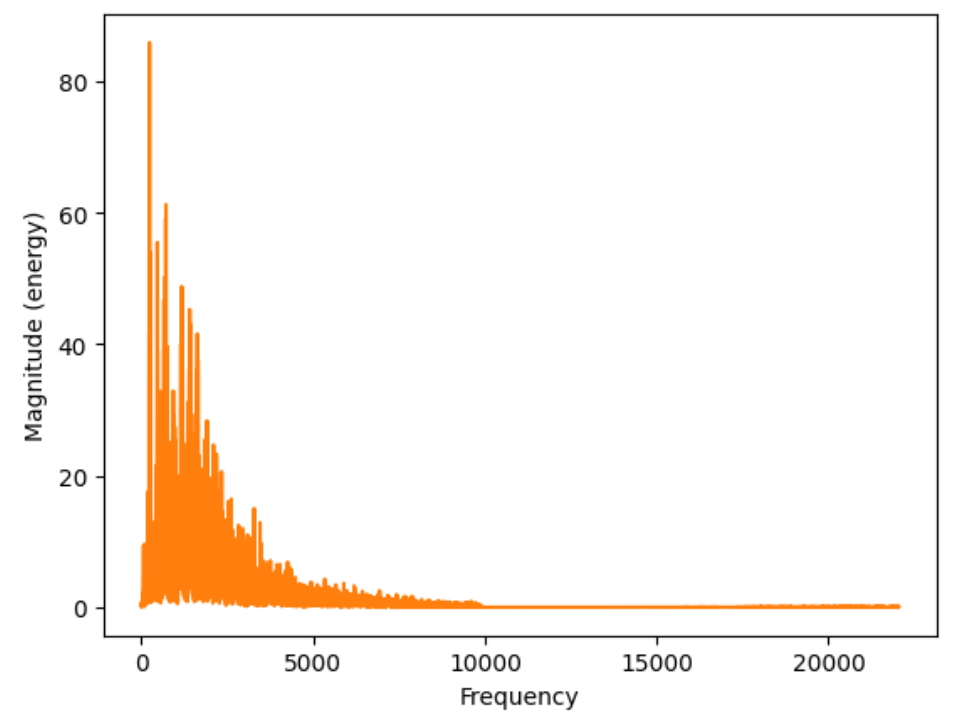
\includegraphics[width=0.7\linewidth]{img/Figure1.jpg}
  \caption{Magnitude spectrum of the chosen part of the recording}
\end{figure}

\newpage
To focus on the frequencies with the highest magnitudes, we analyze the frequencies between 0 Hz and 1750 Hz and display only the magnitudes that exceed 35. For this, we add the following to our code:

\lstinputlisting[language=Python]{py/spectrum_2.py}

We now obtain this spectrum:
\begin{figure}[H]
  \centering
  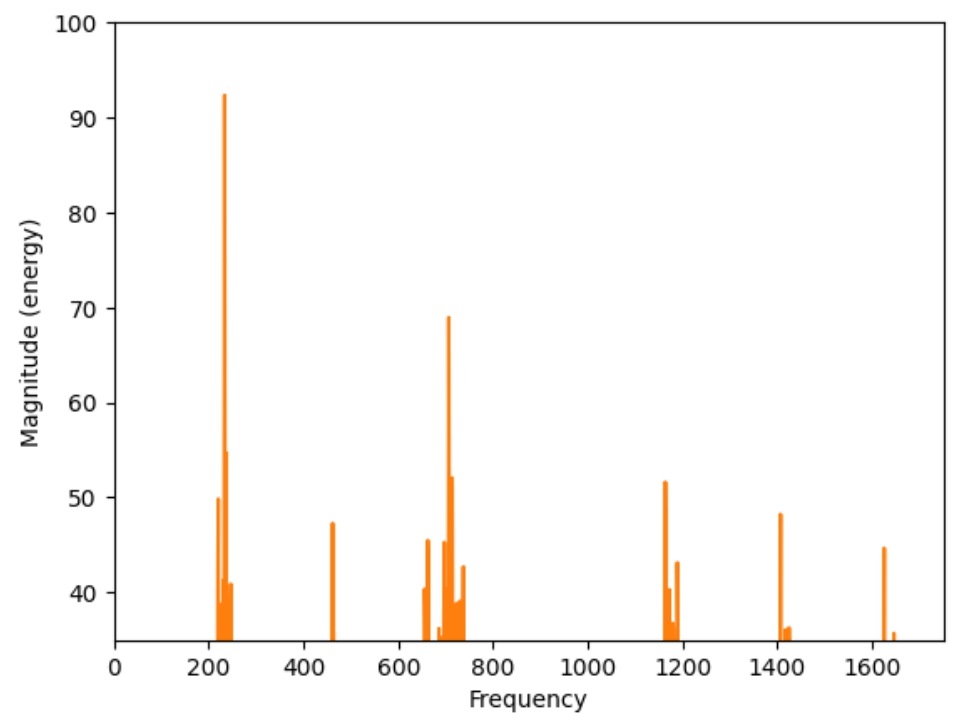
\includegraphics[width=0.7\linewidth]{img/Figure2.jpg}
  \caption{Parameterized magnitude spectrum}
\end{figure}

Now that the spectrum is properly parameterized, we can determine the number L of significant sinusoidal components without any issues. Indeed, \textbf{L=6} as shown by the 6 peaks above.

\newpage
\section{Determination of the frequencies $f_l$}
Next, we seek to determine the specific frequency components $f_l$ that we need to eliminate in order to hear the commentators.

To do this, we will place points on our curve by trial and consider them as value readings. Here is the code that allows us to do this:

\lstinputlisting[language=Python]{py/spectrum_3.py}

We now obtain this spectrum:

\begin{figure}[H]
  \centering
  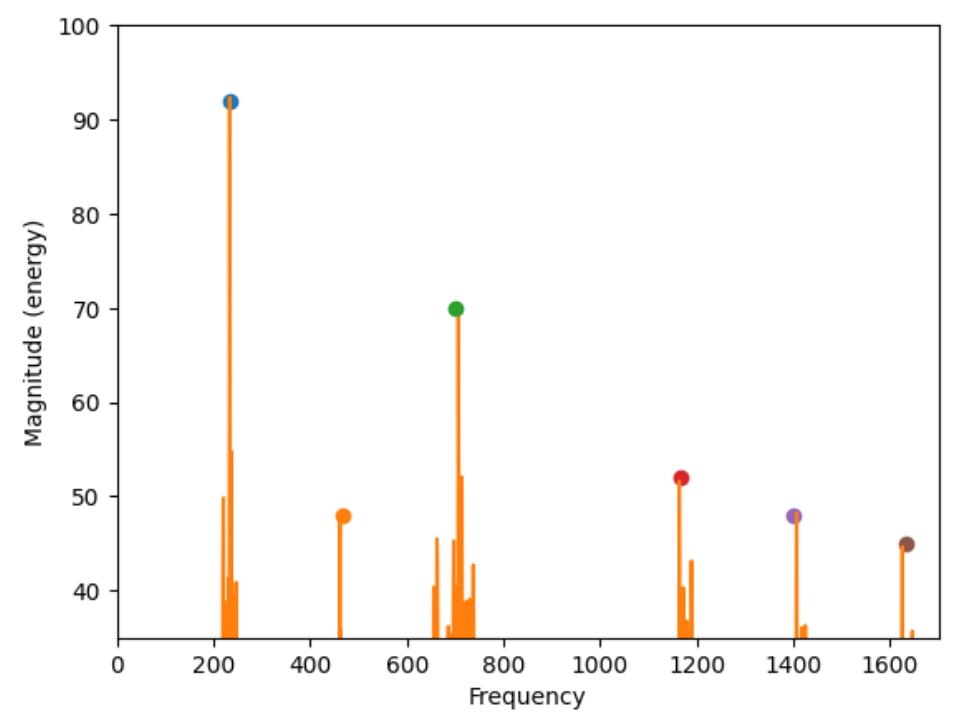
\includegraphics[width=0.7\linewidth]{img/Figure3.jpg}
  \caption{Parameterized magnitude spectrum with value readings}
\end{figure}

The code displays:
"Here is the list of frequencies (they have been normalized to be multiples of the fundamental frequency): [233, 466, 699, 1165, 1398, 1631] \newline
The absence of the frequency 932 Hz is notable."

We now have our specific frequency components $f_l$: \textbf{233 Hz, 466 Hz, 699 Hz, 1165 Hz, 1398 Hz, and 1631 Hz.}

It can be noted, as highlighted by the code, that we have a fundamental frequency of 233 Hz and its harmonics (the frequency being an integer multiple of the fundamental frequency).

\section{Approximate determination of m}
To determine the value of m, we will start from a rejected bandwidth value that we will use. The formula for the width of the rejected band is presented below:

\begin{figure}[H]
  \centering
  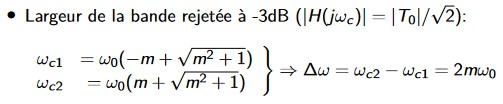
\includegraphics[width=0.7\linewidth]{img/course_excerpt.jpg}
  \caption{Excerpt from Chapter 2: Second-order filters - S4 Electronics Course}
\end{figure}

We have:
$$\Delta\omega = \omega_{c2} - \omega_{c1} = 2m\omega_{0}$$
Which allows us to express $m$ as:
\textbf{$$m = \frac{2\Delta\omega}{\omega_{0}}$$}

From graphical reading, we determine the rejected bandwidths around our specific frequency components $f_l$ as follows:
\begin{enumerate}
    \item 233 Hz: 80 Hz => m $\approx \frac{2\Delta\omega}{\omega_{0}}$ $\approx$ 0.68
    \item 466 Hz: 10 Hz => m $\approx \frac{2\Delta\omega}{\omega_{0}}$ $\approx$ 0.04
    \item 699 Hz: 90 Hz => m $\approx \frac{2\Delta\omega}{\omega_{0}}$ $\approx$ 0.25
    \item 1165 Hz: 45 Hz => m $\approx \frac{2\Delta\omega}{\omega_{0}}$ $\approx$ 0.08
    \item 1398 Hz: 33 Hz => m $\approx \frac{2\Delta\omega}{\omega_{0}}$ $\approx$ 0.04
    \item 1631 Hz: 30 Hz => m $\approx \frac{2\Delta\omega}{\omega_{0}}$ $\approx$ 0.04
\end{enumerate}

\newpage
\section{Implementation of the filter}
We have now determined the parameters of the different filters. It is noteworthy that we will implement a filter for each value of $\omega_0$.
To summarize: \\
$T_0$ = 1, $\omega_0$ = [233, 466, 699, 1165, 1398, 1631], m = $\frac{2\Delta\omega}{\omega_{0}}$.

\subsection{Choice of a notch filter topology} 
To compare the different filters, we present their main characteristics in a table (All the information presented here comes from the Jupyter Notebooks and LTSpice simulations related to each filter).
\begin{figure}[H]
\begin{tabular}{|l|l|l|}
\hline
Filter & RLC Filter & Passive Twin T Filter \\ \hline
Diagram & 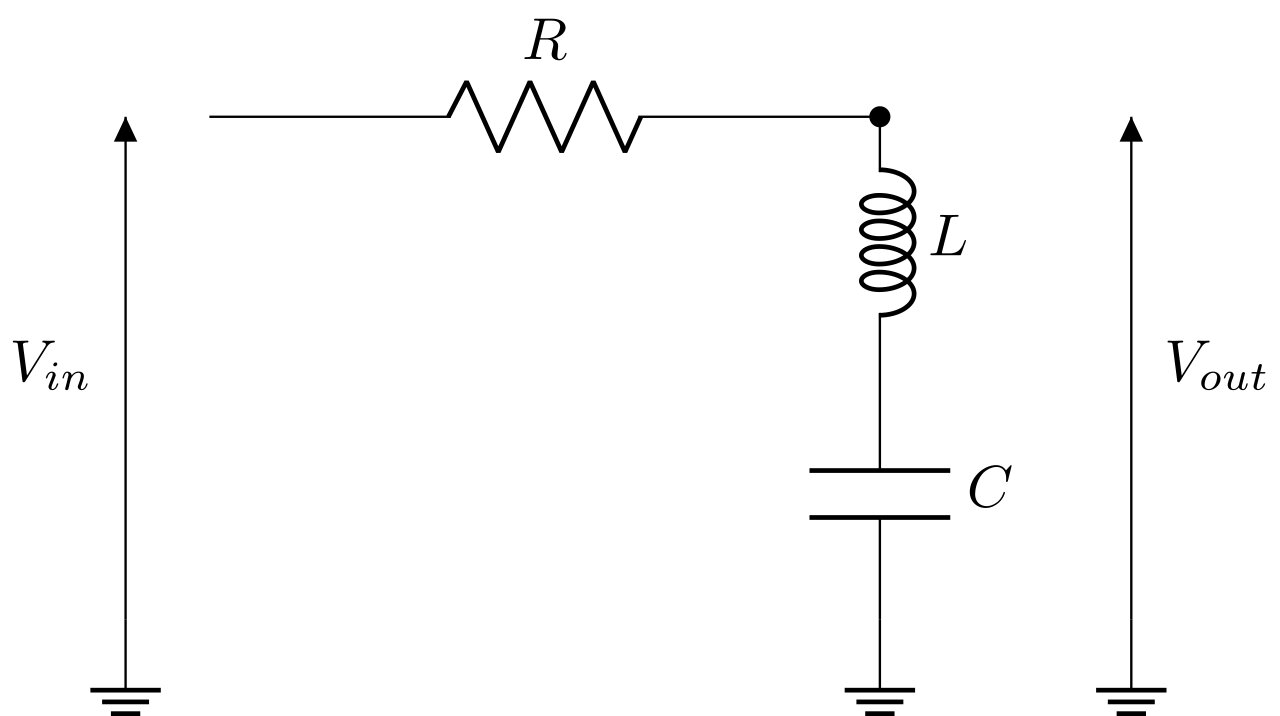
\includegraphics[height=4cm]{img/RLC.jpg} & 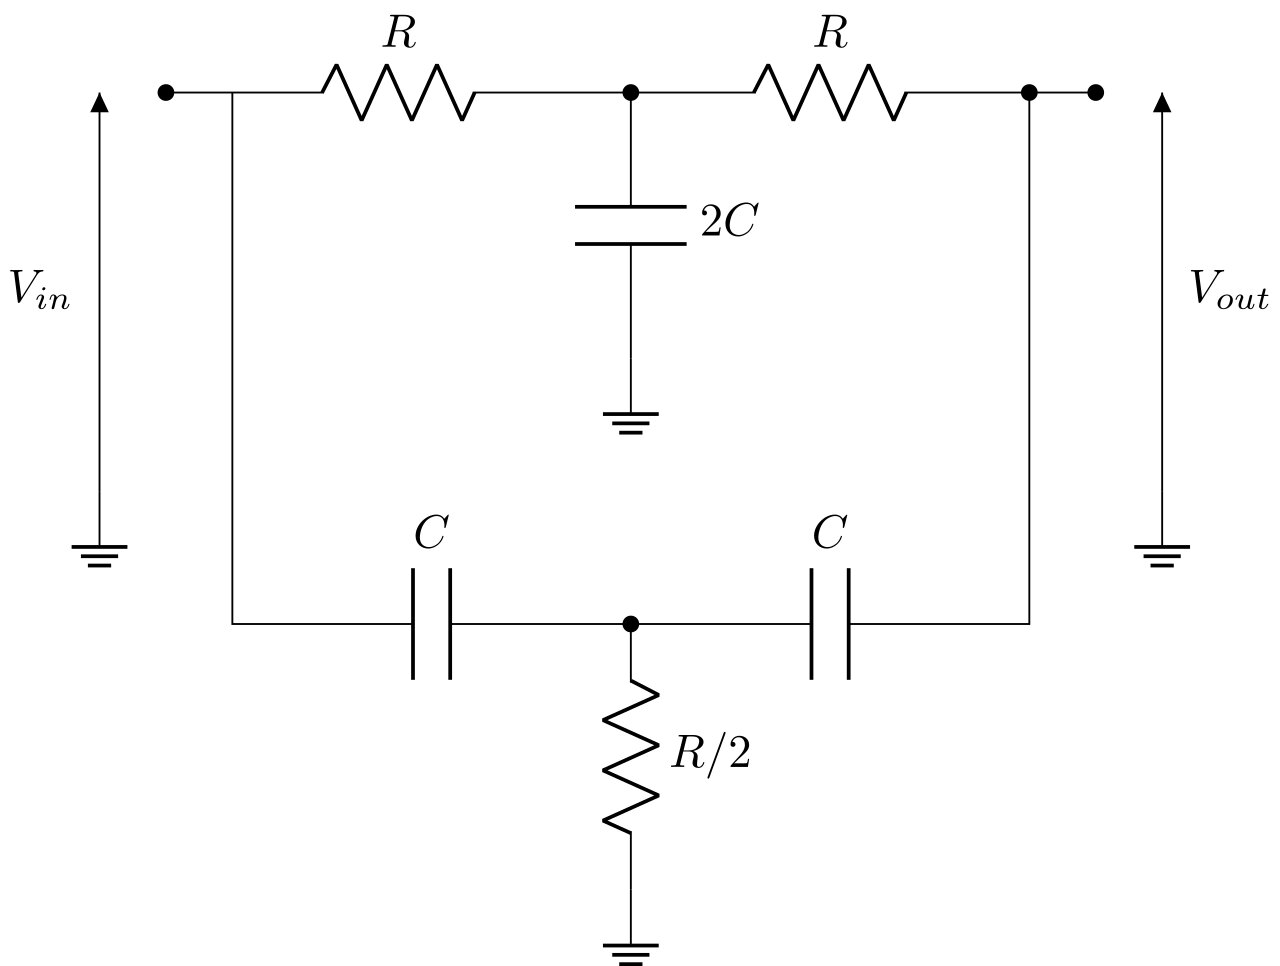
\includegraphics[height=4cm]{img/twin_T.jpg}\\ \hline
Transfer function & $H(p)=\frac{1+LCp^2}{LCp^2+RCp+1}$ & $H(p)=\frac{(RC)^2p^2+1}{(RC)^2p^2+2RCp+1}$ \\ \hline
Comment & \begin{tabular}[c]{@{}l@{}}The filter model is very interesting and\\ easily manipulable, but\\ unfortunately, the internal resistance of the\\ coil disrupts the model and makes it\\ incorrect.\end{tabular} & \begin{tabular}[c]{@{}l@{}}The filter model shows that the damping\\ coefficient m is fixed.\\ This prevents us from choosing the bandwidth,\\ so this filter is not retained.\\ (Here our transfer function is probably\\ incorrect based on our tests, but it seems evident\\ that m will be constant.)\end{tabular} \\ \hline
\end{tabular}
\end{figure}

\begin{figure}[H]
\begin{tabular}{|l|l|l|}
\hline
Filter & Active Twin T Filter & Active Bainter Filter \\ \hline
Diagram & 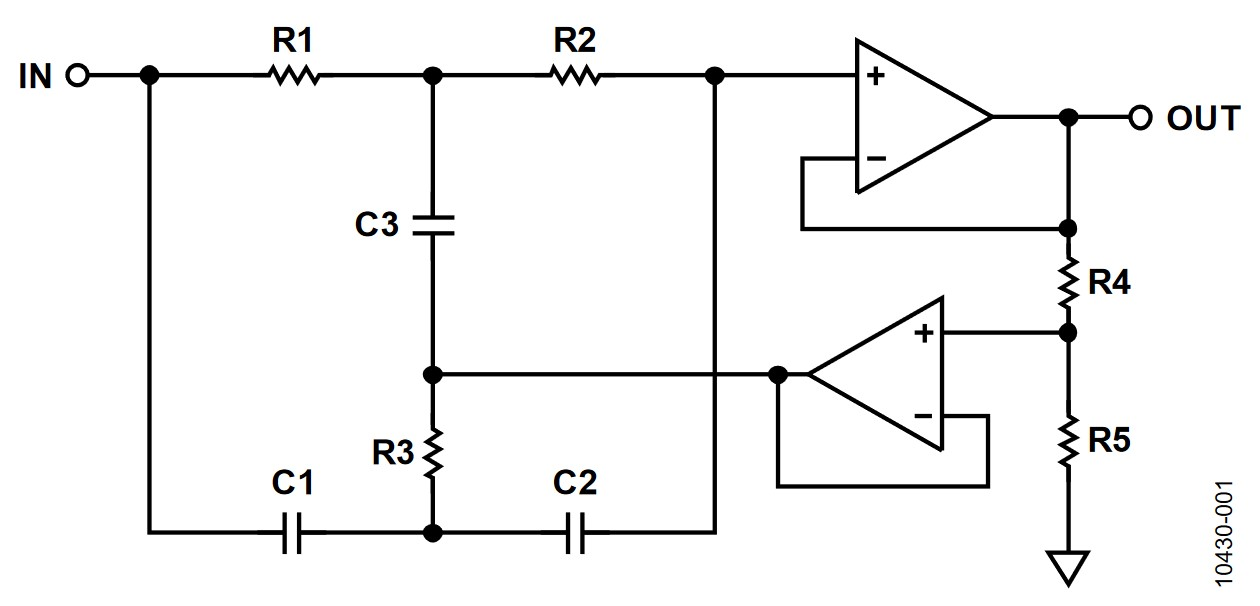
\includegraphics[height=3.45cm]{img/twin_T_active.jpg} & 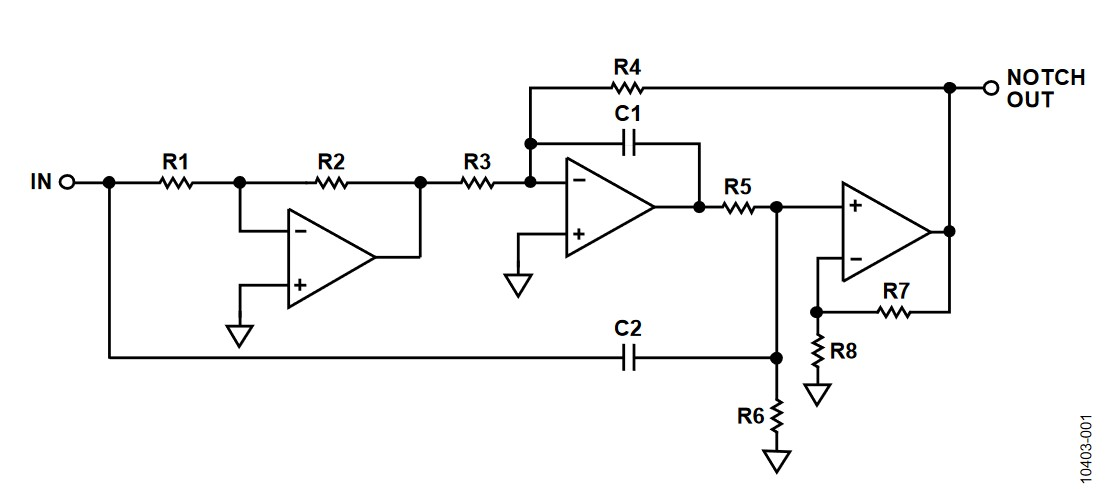
\includegraphics[height=3.05cm]{img/bainter_active.jpg}\\ \hline
Transfer function & $H(p)=\frac{p^2+(\frac{1}{RC})^2}{p^2+p(\frac{1}{RC})(\frac{4}{1+\frac{R5}{R4}})+(\frac{1}{RC})^2}$ & $H(p)= H*\frac{p^2+2w_z}{p^2+\frac{w_0}{Q}+w_0^2}$ \\ \hline
Comment & \begin{tabular}[c]{@{}l@{}}This filter seems to be the best\\ compromise; no real\\ complaints can be made about it.\end{tabular} & \begin{tabular}[c]{@{}l@{}}This filter, although very powerful, is hard to\\ tune, and inconsistencies are observable in\\ certain parts of the filter during the simulation.\end{tabular} \\ \hline
\end{tabular}
\end{figure}

Following this analysis, the filter that seems most appropriate for our project is the \textbf{Active Twin T}.

\subsection{Determination of electronic components}
To determine the electronic components necessary for the implementation of the filter, we use the code below.

(The various parameters are displayed in comments at the bottom of the code).
\lstinputlisting[language=Python]{py/compu.py}

\subsection{LTSpice Test of the chosen cascade of filters}
To perform an LTSpice simulation of our technical solution, we create a filter for each specific frequency component $f_l$ and cascade them.

\begin{figure}[H]
  \centering
  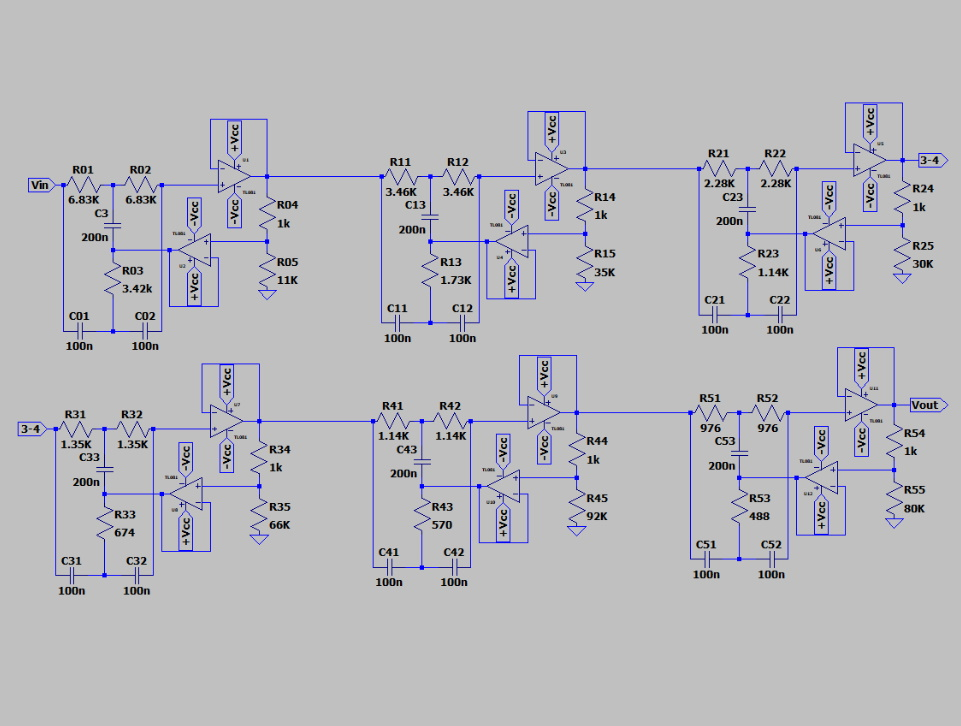
\includegraphics[width=0.7\linewidth]{img/LTSpice_circuit.jpg}
  \caption{Circuit created in LTSpice}
\end{figure}

\newpage
To verify the correct operation of the circuit, we perform a spectral analysis via FFT.
\begin{figure}[H]
  \centering
  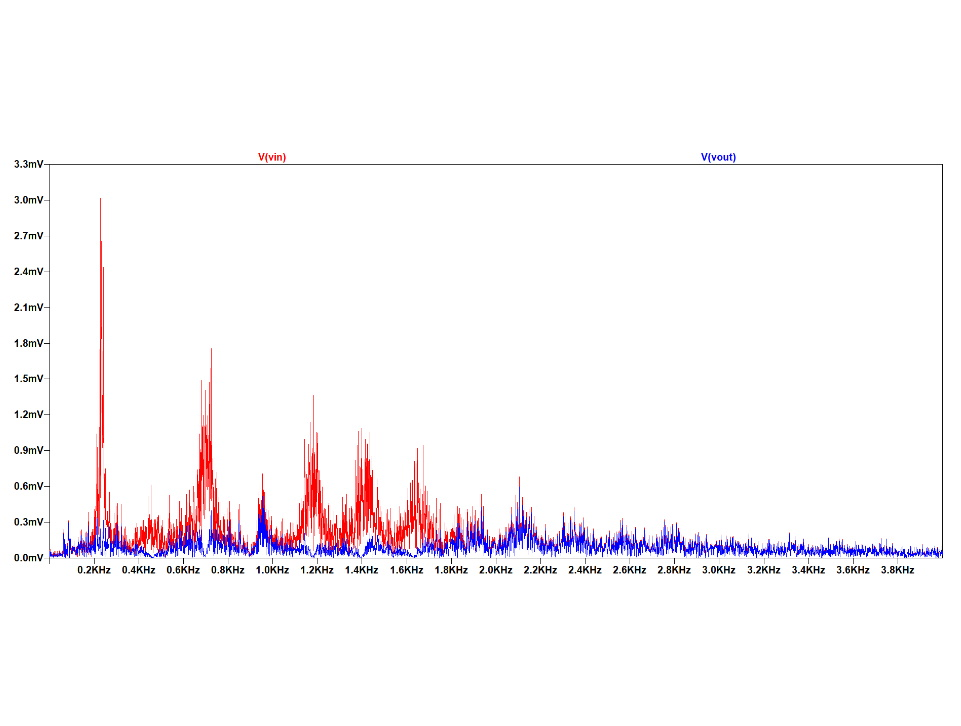
\includegraphics[width=0.7\linewidth]{img/fft_analysis.jpg}
  \caption{Spectral analysis via FFT}
\end{figure}

When we look at the analysis, we see that we have successfully removed the magnitude peaks specific to our "vuvuzela-only" recording. The FFT analysis allows us to conclude that the filter works well!

\newpage
\section{Conclusion}
Through this project, we have successfully implemented a filter that removes the "Vuvuzela" noise present in the audio signal, significantly improving the intelligibility of the commentators' voices. We also demonstrated how to approach a problem involving sound filtering by analyzing the audio signal, determining significant frequency components, and finally implementing a cascading series of notch filters to target these frequencies. Our solution is a practical demonstration of the principles of signal processing in audio engineering.
